\documentclass[11pt]{amsart}
\usepackage{geometry}                % See geometry.pdf to learn the layout options. There are lots.
\geometry{letterpaper}                   % ... or a4paper or a5paper or ... 
%\geometry{landscape}                % Activate for for rotated page geometry
%\usepackage[parfill]{parskip}    % Activate to begin paragraphs with an empty line rather than an indent
\usepackage{graphicx}
\usepackage{amssymb}
\usepackage{epstopdf}
\usepackage{tikz}
\usetikzlibrary{automata}
\usetikzlibrary{positioning}

\DeclareGraphicsRule{.tif}{png}{.png}{`convert #1 `dirname #1`/`basename #1 .tif`.png}

\title{Brief Article}
\author{The Author}
%\date{}                                           % Activate to display a given date or no date

\begin{document}

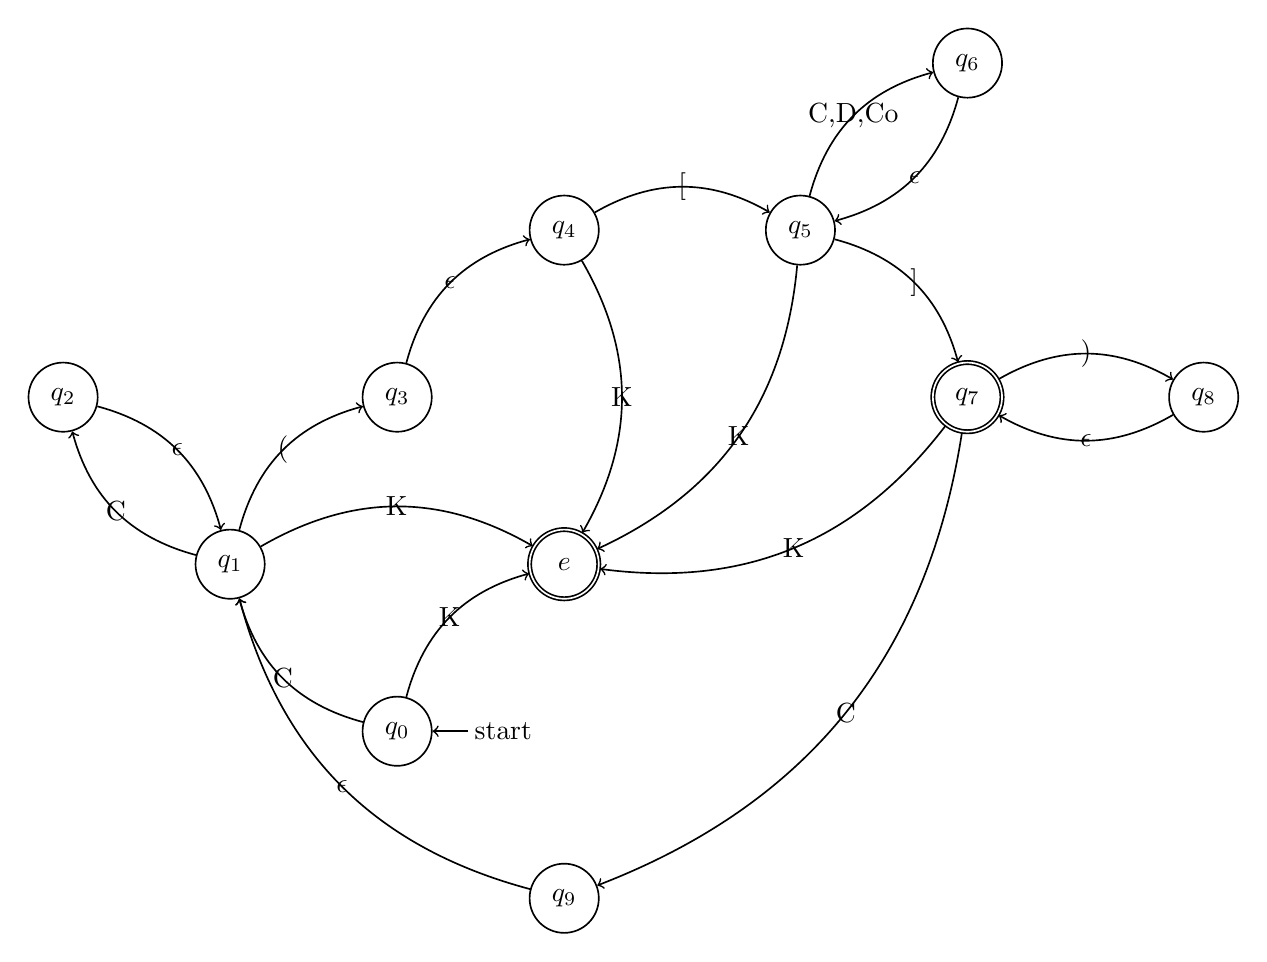
\begin{tikzpicture}[node distance=3cm, on grid, semithick, inner sep= 2pt]%, bend angle=45]

\node [state] (q_1) {$q_1$};
\node [initial right, state, below right = of q_1] (q_0) {$q_0$};
\node [state] (q_2) [above left = of q_1]{$q_{2}$};
\node [state] (q_3) [above right= of q_1]{$q_3$};
\node [state] (q_4) [above right = of q_3]{$q_4$};
\node [state] (q_5) [right=of q_4] {$q_5$};
\node [state] (q_6) [above right=of q_5] {$q_6$};
\node [state, accepting] (q_7) [below right=of q_5] {$q_7$};
\node [state, accepting] (q_e) [below right= of q_3] {$e$};
\node [state] (q_8) [right =of q_7] {$q_8$};
\node [state] (q_9) [below right=of q_0] {$q_9$};

\path [->] 
	      (q_0) [bend left] edge node {C} (q_1)
	      (q_0) edge node {K} (q_e)
               (q_1) edge node {K}(q_e)
               (q_1) [bend left] edge  node {(}(q_3)
               (q_1) [bend left] edge  node {C}(q_2)
               (q_2) [bend left] edge  node {$\epsilon$}(q_1)
               (q_3) [bend left] edge  node {$\epsilon$}(q_4)
               (q_4) edge node {K}(q_e)
               (q_4) edge  node {[}(q_5)
               (q_5) edge node {C,D,Co} (q_6)
               (q_6) edge node {$\epsilon$} (q_5)
               (q_7) [bend left] edge node {)}(q_8)
               (q_8) [bend left] edge node {$\epsilon$}(q_7)
                (q_5) [bend left] edge node {]}(q_7)
	       (q_5) edge node {K}(q_e)
	       (q_7) edge node {K}(q_e)
	       (q_7) edge node {C}(q_9) 
	       (q_9) edge node {$\epsilon$}(q_1) 
	       ;


\end{tikzpicture}

\begin{center}
\begin{tabular}{|l|l|l|} \hline
function & diagram & comment \\ \hline
    start & - &\\
    scenario & $q_0$ &  expect character, set $1^{st}$ scenario name char\\
    scenario & $q_1, q_2 $ & accumulate scenario name\\
    scenario & $q_3$ & push node stack, clear name\\
    start\_params & $q_4$& expect '['\\
    params & $q_5, q_6$& accumulate scenario parameters\\
    end\_params & $q_7,$& set attr parameters stack top, clear params\\
    end\_params &$q_8$& collapse parens: stack pop; add child; clear name, pars\\
    end\_params &$q_9$& add char to scenario name\\
    error & $e$& raise exception \\
\hline
\end{tabular}
\end{center}
$$\Sigma = \{\epsilon,a-z0-9][)(,\}.\ \epsilon\text{ is the empty string}$$

Abbreviations:
\begin{center}
\begin{tabular}{ll}
C & \{a-z\}\\
Co& , \\
D  & \{0-9\}\\
%  $\sim$\{\dots\} & $\Sigma$\textbackslash \{\dots\} \\
K & $\Sigma$\textbackslash \{all other out symbols for the node\} \\
\end{tabular}
\end{center}




\end{document}  